% --------------------------------------------------------------
% This is all preamble stuff that you don't have to worry about.
% Head down to where it says "Start here"
% --------------------------------------------------------------
 
\documentclass[12pt]{article}
 
\usepackage[margin=1in]{geometry} 
\usepackage{amsmath,amsthm,amssymb}
\usepackage{graphicx}
\usepackage{float}
\usepackage{listings}
\usepackage{url}
\usepackage{color}
\usepackage{enumerate}
\usepackage{flushend}
\usepackage{graphicx}

\usepackage[numbers]{natbib}

\newcommand{\N}{\mathbb{N}}
\newcommand{\Z}{\mathbb{Z}}
\newcommand\floor[1]{\lfloor#1\rfloor}
\newcommand\ceil[1]{\lceil#1\rceil}

\newenvironment{theorem}[2][Theorem]{\begin{trivlist}
\item[\hskip \labelsep {\bfseries #1}\hskip \labelsep {\bfseries #2.}]}{\end{trivlist}}
\newenvironment{lemma}[2][Lemma]{\begin{trivlist}
\item[\hskip \labelsep {\bfseries #1}\hskip \labelsep {\bfseries #2.}]}{\end{trivlist}}
\newenvironment{exercise}[2][Exercise]{\begin{trivlist}
\item[\hskip \labelsep {\bfseries #1}\hskip \labelsep {\bfseries #2.}]}{\end{trivlist}}
\newenvironment{reflection}[2][Reflection]{\begin{trivlist}
\item[\hskip \labelsep {\bfseries #1}\hskip \labelsep {\bfseries #2.}]}{\end{trivlist}}
\newenvironment{proposition}[2][Proposition]{\begin{trivlist}
\item[\hskip \labelsep {\bfseries #1}\hskip \labelsep {\bfseries #2.}]}{\end{trivlist}}
\newenvironment{corollary}[2][Corollary]{\begin{trivlist}
\item[\hskip \labelsep {\bfseries #1}\hskip \labelsep {\bfseries #2.}]}{\end{trivlist}}
 \usepackage{color}

\definecolor{dkgreen}{rgb}{0,0.6,0}
\definecolor{gray}{rgb}{0.5,0.5,0.5}
\definecolor{mauve}{rgb}{0.58,0,0.82}

\lstset{frame=tb,
  language=python,
  aboveskip=3mm,
  belowskip=3mm,
  showstringspaces=false,
  columns=flexible,
  basicstyle={\small\ttfamily},
  numbers=none,
  numberstyle=\tiny\color{gray},
  keywordstyle=\color{blue},
  commentstyle=\color{dkgreen},
  stringstyle=\color{mauve},
  breaklines=true,
  breakatwhitespace=true,
  tabsize=3
}
 
\begin{document}
 
% --------------------------------------------------------------
%                         Start here
% --------------------------------------------------------------
 
%\renewcommand{\qedsymbol}{\filledbox}
 
\title{Project 01}%replace X with the appropriate number
\author{Aravindh Kuppusamy, Deepak Sharma, Karan Jariwala\\ %replace with your name
CSCI 630-01 Foundations of Intelligent Systems} %if necessary, replace with your course title
 
\maketitle
 
\begin{section}{Problem Definition} 
\subsection{State}
Configuration of all possible positions in the maze along with the dice orientation at each possible position. If the width of the maze is W and height of the maze is H, then W*H positions are possible. Out of these positions, let O positions be obstacles and hence, the dice can't be moved to those locations. 20 orientations of dice are possible for each non-goal position and 4 orientations for goal position. Hence the size of the state space is:
\[
 {\mathbf{State space Size: (((W*H)-O-1)*20) + (1*4)}} 
\]

\subsection{Successor Function}
Successor function generates all the possible moves from a given state. Here, Successor function generates states which represents both the dice location in the maze and its orientation. So, the successor function for the problem is legal moves in both maze and dice in same direction.
\subsubsection{Legal positions in Maze for successor states}
The possible moves include moving in four directions (Top, Bottom, Right, and Left) to the adjacent position with step cost as 1. But if the resulting position is an obstacle, then the move is not legal. So the legal moves would be all possible moves without illegal ones.
\subsubsection{Legal orientations of Dice for successor states}
The possible orientations include turning in four directions (Top, Bottom, Right, and Left) by one step. But if the resulting position is an orientation of dice with top value = 6 for a non-goal state and top value != 1 for goal state, then the move is not legal. So the legal moves would be all possible moves without illegal ones.

\subsection{Goal test}
Whether the Goal position in the maze has been reached with the dice orientation having top value = 1. 
\subsection{Path Cost}
Total number of moves till the current state.



\end{section}

 \begin{section}{Heuristics}
 \label{heuristics}
 \subsection{MANHATTAN DISTANCE}
 Manhattan distance is the sum of the vertical and horizontal distances between two points. If (x1, y1) and (x2, y2) are the two points then Manhattan distance between them is 
\begin{equation}\mathbf{ d= |x_1-x_2|+|y_1-y_2|} \end{equation}  
\par Since the problem state is a grid and we cannot move in other than the 4 directions, and by also relaxing the constraint of obstacles through which we can’t pass, Manhattan distance is the shortest path and hence it’s optimal.

\subsubsection{Proof for Admissibility}
A heuristic is admissible if estimated cost is never greater than the actual cost from the current state to goal state\cite{Russell:2003:AIM:773294}.
\par
For a given state at location $\mathbf{(x_s, y_s)}$ and goal location $\mathbf{(x_g, y_g)}$, the distance we have to travel is at least $\mathbf{|x_s - x_g| + |y_s - y_g|}$ since we can move only in horizontal and vertical directions. We are also relaxing the constraint of obstacles and dice configurations.
Proof by Contradiction:
\par
Base Case:
\[
 {\mathbf{h(goal) = 0}} 
\]

Let C be the minimum actual cost for traveling from start state to goal state. .i.e., at least C steps are required for traveling from start state to goal state Assume, the actual cost(C):
\begin{equation}\mathbf{ \mathbf{C < h(start)}} \end{equation}  

For each action we perform, the step cost will be just 1. So heuristics for the successor state will reduce by just 1.
\[
 {\mathbf{Cost(parent -> child) = 1}} 
\]
Hence,
\[
 {\mathbf{h(successor) = h(parent) - 1}} 
\]
Since, at least C steps are required for traveling from start state to goal state,
\[
 {\mathbf{h(goal) >= h(start) - C}} 
\]
\[
 {\mathbf{h(goal) >= h(start) - C > 0}} 
\] 

From 2
\[
 {\mathbf{h(goal) > 0}} 
\] 
This contradicts the base case and so our assumption is wrong.
Therefore, 
\[
 {\mathbf{C >= h(start)}} 
\] 

Hence, we conclude that Manhattan distance heuristics is admissible.


\subsection{DIAGONAL DISTANCE}Diagonal distance is the sum of the number of diagonal steps possible and the remaining straight line distance between two points. In diagonal Heuristic, the cost is generated while considering the horizontal, vertical and diagonal paths toward the goal which means that it can look up the path or a state in 8 directions while calculating the heuristic cost.
If $\mathbf{(x_1, y_1)}$ and $\mathbf{(x_2, y_2)}$ are the two points then Diagonal distance between them is:
\[
 {\mathbf{d_x=|x_1-x_2|}} 
\]
\[
 {\mathbf{d_y=|y_1-y_2|}} 
\]

\begin{equation} \mathbf{d=\sqrt{2}*min(d_x,d_y)+|d_x-d_y|} \end{equation}  
\subsubsection{Proof for Admissibility}

\begin{figure}[H]
\label{triangle}
\begin{center}
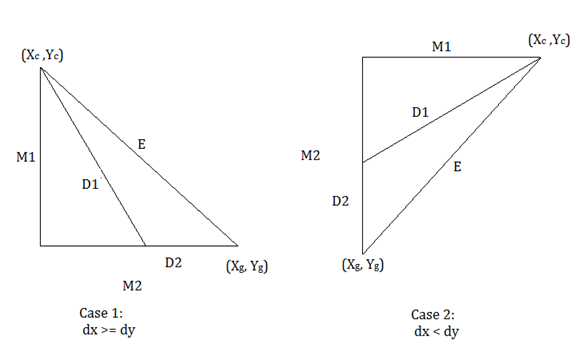
\includegraphics[width=5.0in, scale=0.25]{triange.png}
\caption{Left triangle represents the case when $\mathbf{dx >= dy}$ and right triangle represents the case when $\mathbf{dx < dy}$ }
\end{center}
\end{figure}

For a given set of positions $\mathbf{(x_1, y_1)}$ and $\mathbf{(x_2, y_2)}$, there are two cases possible as shown in the figure 1:

 1) $\mathbf{dx >= dy}$ or \par2) $\mathbf{dx < dy}$

For the given current node $\mathbf{(x_c, y_c)}$ and the goal node $\mathbf{(x_g, y_g)}$, the diagonal heuristic $\mathbf{h_{diagonal} = D1 + D2}$. Now by triangle inequality,

 \[
 {\mathbf{M1 + ( M2 - D2 ) >= D1}} 
\]
\[
 {\mathbf{M1+ M2 >= D1 + D2.}} 
\]

Here, $\mathbf{M1 + M2}$ is the Manhattan heuristics for the point $\mathbf{(x_c, y_c)}$. So, Euclidean distance is always lesser than or equal to Manhattan distance.
From above statement, we can say that for any point P in real coordinate system,
 \[
 {\mathbf{h_{diagonal}(P) <= h_{manhattan}(P)}} 
\]
i.e., Manhattan heuristics dominates diagonal heuristics.  Since, Manhattan heuristics dominates diagonal heuristics and also Manhattan heuristics is admissible, we can infer that diagonal heuristics is also admissible.

\subsection{EUCLIDEAN DISTANCE}
Euclidean distance is the distance of the straight line that connects two points. If $\mathbf{(x_1, y_1)}$ and $\mathbf{(x_2, y_2)}$ are the two points then Euclidean distance between them is:
\begin{equation} \mathbf{d=\sqrt{(x_1-x_2)^2+(y_1-y_2)^2}} \end{equation}  

\subsubsection{Proof for Admissibility}
According to triangle inequality, the sum of two sides is always greater than or equal to the third side.
\par
Euclidean distance is the hypotenuse (third side) in the triangle formed by two sides dx and dy in Manhattan distance, where
 \[
 {\mathbf{dx =|x_1-x_2|  } \quad \textrm{and} \quad \mathbf{dy =|y_1-y_2| } } 
\]

So, Euclidean distance is always lesser than or equal to Manhattan distance. From above statement, we can say that,

 \[
 {\mathbf{h_{euclidian}(P) <= h_{manhattan}(P)}} 
\]

i.e., Manhattan heuristics dominates Euclidean heuristics.  Since, Manhattan heuristics dominates Euclidean heuristics and also Manhattan heuristics is admissible, we can infer that Euclidean heuristics is also admissible.


\subsection{FANCY MANHATTAN DISTANCE}
Fancy Manhattan heuristics is nothing but sum of Manhattan distance and a reward $\mathbf{\alpha = -0.5}$ for a state.
 If the current state\textsc{\char13}s position is $\mathbf{(x_c, y_c)}$ and the goal state\textsc{\char13}s position is $\mathbf{(x_g, y_g)}$, then horizontal and vertical distances between them are
 \[
 {\mathbf{dx =|x_g-x_c|  }  \quad \textrm{and} \quad \mathbf{dy =|y_g-y_c| } } 
\]
Reward comes into play if $\mathbf{dx <=1}$ or $\mathbf{dy <= 1}$. We add reward to heuristics if we rotate the dice from current location $\mathbf{(x_c, y_c)}$ to the goal location $\mathbf{(x_g, y_g)}$ and if it is passing goal test. We perform four types of rotations for calculating dice face value:
\par
If $\mathbf{dy<=1}$ then:
\begin{enumerate}
\item{if $\mathbf{dx>0}$ then, rotate the dice $\mathbf{|dx|mod 4}$ time in right direction}
\item{if $\mathbf{dx<0}$ then, rotate the dice $\mathbf{|dx|mod 4}$ time in left direction.}
\end{enumerate}
Now, Rotate the dice by dy steps in corresponding direction.
\par
Similarly if $\mathbf{dx<=1}$  then:
\begin{enumerate}
\item{
if $\mathbf{dy>0}$ then rotate dice $\mathbf{|dy| mod 4}$ times in south direction }
\item{
if $\mathbf{dy<0}$ or $\mathbf{|dy|mod 4}$ times in North direction.}
\end{enumerate}
Now, Rotate the dice by dx steps in corresponding direction.\par
\textbf{Note:} This operation is not computational heavy since maximum value by mod 4 operation we can get is 3. 
\par
After performing rotations, If face value is 1 then :
\par
 \[
 {\mathbf{h_{fancyManhattan}(n) = h_{manhattan}(n) + \alpha}} 
\]
\par
For other cases:
\par
 \[
 {\mathbf{h_{fancyManhattan}(n) = h_{manhattan}(n) }} 
\]

\subsubsection{Proof for Admissibility}

Here, we are actually either subtracting the Manhattan heuristics by 0.5 as per the above conditions or we just return Manhattan heuristics. So, the fancy Manhattan heuristics is less than or equal to Manhattan heuristics. We know that Manhattan distance is admissible. 
Hence, the fancy Manhattan heuristics is also admissible since it never over predicts the cost than Manhattan heuristics.

\end{section}
 
\begin{section}{Performance metrics}

\begin{figure}[H]
\label{map1}
\begin{center}
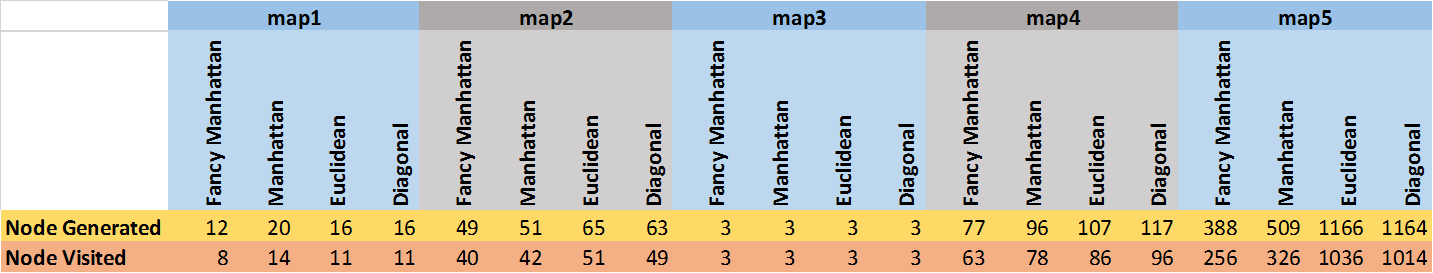
\includegraphics[width=7.0in]{table.png}
\caption{Performance of various Heuristics for Map(1-5)  }
\end{center}
\end{figure}


\begin{figure}[H]
\label{map1}
\begin{center}
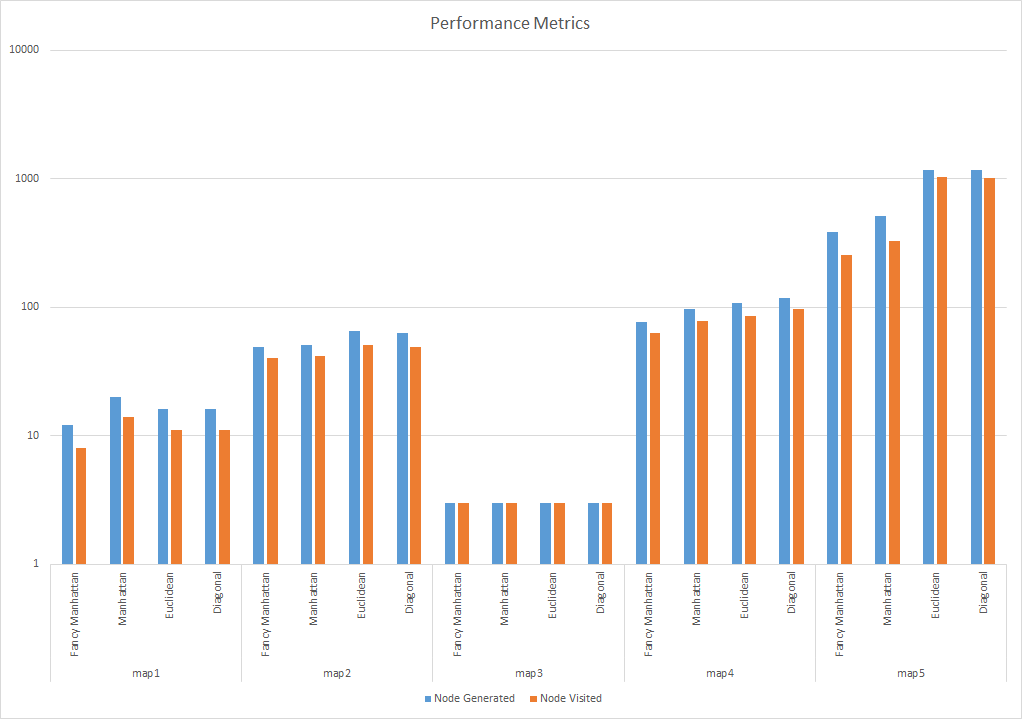
\includegraphics[width=7.0in]{graphImage.png}
\caption{Performance of various Heuristics for Map(1-5)  }
\end{center}
\end{figure}



\end{section}
 
\begin{section}{Discussion}
 
  After conducting experiments by executing the A* search algorithm for given problem we have found that our suggested fancy Manhattan and Manhattan heuristic have performed better than euclidean and diagonal heuristic. As we discussed in the section \ref{heuristics}, Manhattan heuristic is a dominant heuristic over euclidean and diagonal heuristic because: 
 \[
 {\mathbf{h_{Manhattan}(n)>h_{Euclidean}(n) \quad \textrm{and} \quad h_{Manhattan}(n)>h_{Diagonal}(n) }}
\]
 \par For the given problem the dice is only allowed to move in north, south, east and west direction. Hence in the ideal case dice has to take at least $\mathbf{h_{Manhattan}(S)}$ steps for solving the maze. However, the estimations provided by the Euclidean and Diagonal heuristic on  average are much lesser than actual path as they calculate the distances of diagonal paths, which dice is not allowed to take, so these estimations are not near to the reality. 
 \par Fancy Manhattan Heuristic has given best result as it reduces the number of nodes explored before reaching to the goal as it gives precedence to the nodes which can take the dice to the goal positions with 1 on the top just by following the path taken by Manhattan Heuristic while calculating estimate.  
\par We came up with many other Heuristics, but either they were not consistent or they were computationally heavy so we didn't use them as they were violating one of the key requirement which has to be a consistent heuristics. Hence a heuristic function apart from being admissible, it shouldn’t be computationally heavy else we might end up doing overall more computation than the dijkstra algorithm. i.e., We might end up with expanding less number of states in A* search algorithm, but will result in increasing the time complexity since for calculating heuristics of each state, we would be expanding the states to give better values.

We noticed that, Fancy Manhattan heuristic is admissible but not consistent. Though it reduces the expanded nodes, it fails to be consistent because in our case, \[\mathbf{h(s) >= c(s,a,g) + h(g)}\]
whereas it should be,
 \[\mathbf{h(s) <= c(s,a,g) + h(g)}\]
Here s is the start state, a is an intermediate state whose dx or dy is less than 2, and g is the goal state.
Since we are reducing the distance by rewarding(adding) a negative value in heuristics only for some positions, it fails to be consistent. But in this game, though it's not consistent, it doesn't result in any issues.
\end{section} 
 
\bibliographystyle{plainnat}
\bibliographystyle{abbrv}


% \bibliographystyle{plainnat}
%\bibliographystyle{abbrv}
\bibliography{homework}
 
\end{document}